\documentclass[11pt,a4paper]{article}
\usepackage[margin=24mm]{geometry}
\usepackage[T1]{fontenc}
\usepackage{lmodern,amsmath,amssymb,graphicx,booktabs,xcolor}
\usepackage{microtype,needspace}
\usepackage[colorlinks=true,urlcolor=blue,linkcolor=blue]{hyperref}
\setlength{\parindent}{0pt}
\setlength{\parskip}{0.55em}
\setlength{\emergencystretch}{2em}
\graphicspath{{figures/}}
\renewcommand{\thefigure}{R\arabic{figure}}
\newcommand{\authornote}[1]{\par\smallskip\noindent
 \colorbox{gray!10}{\parbox{\dimexpr\linewidth-2\fboxsep\relax}{\small
 \textbf{Author-review note.} #1}}\par\smallskip}
\newcommand{\commentheading}[1]{\Needspace{7\baselineskip}\subsection*{Comment #1}}

\begin{document}
\begin{center}
 {\Large\bfseries Response to Referee 1}\par\vspace{0.4em}
 {\normalsize Mixing effects in radiative decays of heavy-strange axial-vector\\
 mesons within light-cone QCD sum rules}\par\vspace{0.3em}
 T. M. Aliev, S. Bilmis, and M. Savci
\end{center}

\authornote{Working draft, 19 October 2026. Statements about manuscript
 additions assume that the accompanying proposed changes have been inserted
 into Prism. The numerical input-sensitivity part of Comment 1 remains
 incomplete; its completion note below must be replaced before submission.}

We thank the referee for the positive assessment of our work and for the
constructive suggestions. We address the three comments below.

\commentheading{1}
\begin{quote}\small\itshape
In describing the approach used to calculate the radiative widths of
axial-vector meson states, the authors refer to their previous work on
estimating the mixing angle of the $^1P_1$ and $^3P_1$ spin states
(Phys. Rev. D 111, No. 1 (2025) 014005). In my view, it would be beneficial
for the reader if the authors briefly outlined this approach and the main
results in the present article, taking into account---however slight---the
changes in the input parameter values (such as the quark condensate
magnitude) used in these studies.
\end{quote}

\textbf{Response.}
We thank the referee for this suggestion. We have added a short account of
the mixing-angle determination after the two-point sum rules for the decay
constants in Section II. In the two-state method of our earlier work,
the angle is obtained by imposing a vanishing off-diagonal spin-one
correlator in the rotated current basis. For the convention used in the
present manuscript,
\begin{equation}
 R(\theta)=\begin{pmatrix}\sin\theta&\cos\theta\\
 \cos\theta&-\sin\theta\end{pmatrix},\qquad
 \bigl[R\widehat{\boldsymbol\Pi}R^T\bigr]_{12}=0.
\end{equation}
With a common Borel and continuum prescription for the matrix entering
the angle extraction, this gives
\begin{equation}
 \tan(2\theta)=-\frac{2\widehat\Pi_{AB}}
 {\widehat\Pi_{AA}-\widehat\Pi_{BB}}.
\end{equation}
The added explanation also makes explicit that this relation does not
require equal physical diagonal correlators. Their difference cancels
when the two inverse-rotation relations are divided. The earlier results,
$\theta_{D_s}=26.6^\circ\pm0.6^\circ$ and
$\theta_{B_s}=38.5^\circ\pm0.1^\circ$, are the external angle inputs
used in the present numerical analysis.

We also clarify a typographical omission in the earlier article: the
normalization factor $1/(m_Q+m_s)$ was included in the calculations,
but was inadvertently omitted from the printed tensor-current definition.
Thus, the normalization used in the two calculations is the same.

The updated QCD inputs are a separate issue. In particular, the light-quark
condensate changes from
$-(1.65\pm0.15)\times10^{-2}\,\mathrm{GeV}^3$ to
$-(0.240\pm0.010)^3\,\mathrm{GeV}^3$ at $1\,\mathrm{GeV}$, while
the central value of $\langle\bar ss\rangle/\langle\bar qq\rangle$
remains $0.80$ and its uncertainty changes from $0.20$ to $0.10$.
The strange-quark mass values are quoted at different scales and must
be compared after consistent scale evolution.

\authornote{Complete this part using the original mixing-angle implementation:
 first reproduce the earlier-input baseline, then repeat with the updated
 condensates and other inputs at consistent scales, holding the OPE and
 auxiliary prescription fixed. Report the resulting angle shifts for both
 sectors and compare them with the quoted uncertainties. No statement that
 the effect is negligible has yet been established. The existing
 $\theta=90^\circ$ decay-constant check does not supply this comparison.}

\commentheading{2}
\begin{quote}\small\itshape
It seems to me that it would be very interesting to obtain---within the
framework of the approach proposed by the authors---the values of the
radiative decay widths into the vector $D_s^*$ and $B_s^*$ meson states.
Of course, the calculation of these widths might well warrant a separate
paper. However, the authors should, in my view, note that measuring
absolute widths is a far more challenging experimental task than
measuring the ratio of radiative decay widths into two different final
states. This holds particularly true for the P-wave states of $B_s$
mesons. One would also expect the ratio of decay probabilities into
$D_s\gamma$ and $D_s^*\gamma$ for the $D_{s1}(2536)$ to depend strongly
on the mixing angle.
\end{quote}

\textbf{Response.}
We thank the referee for this useful suggestion. We agree that ratios
of radiative widths into pseudoscalar and vector final states are
experimentally more accessible than absolute widths, particularly for
the bottom-strange mesons, and may provide complementary information on
the mixing angle.

We are currently preparing a separate study of radiative transitions
into the vector states $D_s^*$ and $B_s^*$. Following the referee's
suggestion, that study will also present the ratios to the pseudoscalar
channels and examine their mixing-angle dependence, including the
$D_{s1}(2536)$ channel. We have added a brief statement at the end of
the Conclusion explaining the experimental motivation and the scope
of this forthcoming study.

\commentheading{3}
\begin{quote}\small\itshape
The decay constants $f_1$ and $f_2$ for the physical states
$D_{s1}(2460)$ and $D_{s1}(2536)$, obtained in the paper as a byproduct,
are of independent interest; they allow for the calculation---within the
factorization approximation---of the ratio of the branching fractions
for the $B$-meson decays into $D_{s1}(2536)D^-$ and
$D_{s1}(2460)D^-$. As evidenced by LHCb results (arXiv:2411.03399),
this ratio is experimentally accessible, given that the branching
fractions for the decays of both $D_{s1}(2460)$ and $D_{s1}(2536)$
into $D_s\pi^+\pi^-$ have already been measured. It would be interesting
to present the dependence of the ratio $f_2/f_1$ on the mixing angle
in the paper.
\end{quote}

\textbf{Response.}
We thank the referee for pointing out this additional use of the decay
constants and the experimental motivation. We have added a figure in
Section III showing $f_1(\theta)$ and $f_2(\theta)$ separately for both
the charm-strange and bottom-strange systems. This displays the quantities
that enter our radiative-decay sum rules and makes their angle dependence
explicit. We supply the requested ratio $f_2(\theta)/f_1(\theta)$ in
Fig.~\ref{fig:response-ratio} of this response. The ratio figure is kept
in the response, while the manuscript contains the individual constants.

Both plots use the same fixed representative QCD and auxiliary inputs
as the radiative-width angular scan. The two-point residues are recomputed
at each angle, and the ratio is formed from the two constants at that
same angle. For these illustrative input choices,
\begin{equation}
 \left.\frac{f_2^{(D_s)}}{f_1^{(D_s)}}\right|_{26.6^\circ}
 \simeq 0.418,\qquad
 \left.\frac{f_2^{(B_s)}}{f_1^{(B_s)}}\right|_{38.5^\circ}
 \simeq 0.166.
\end{equation}
These are fixed-input scan values, rather than separately propagated
predictions for the ratios. The radiative-width scan already includes
the angle dependence of the residues; we have clarified its description
and caption to state this explicitly.

\begin{figure}[tbp]
 \centering
 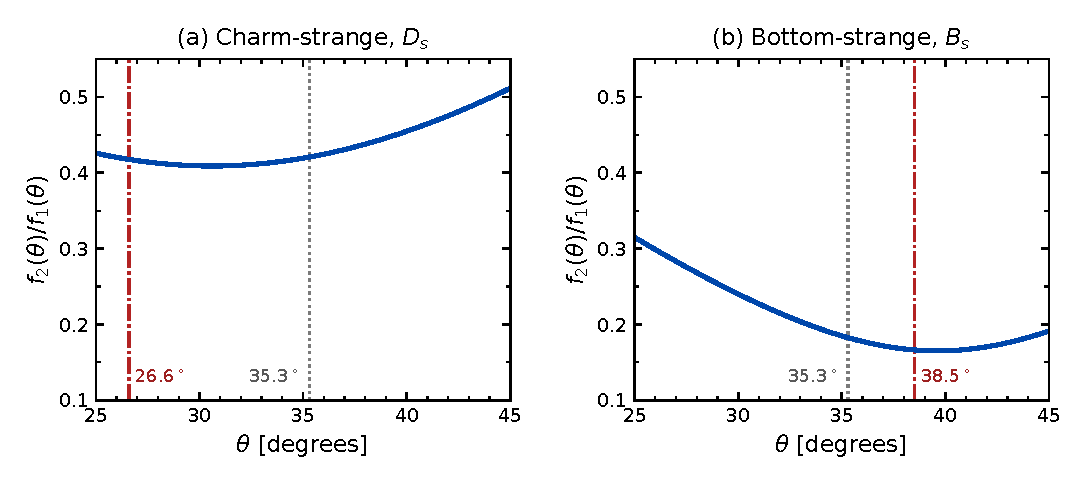
\includegraphics[width=\linewidth]{decay_constant_ratio_vs_theta.pdf}
 \caption{Ratio of the rotated-current decay constants,
 $f_2(\theta)/f_1(\theta)$, for the charm-strange (left) and bottom-strange
 (right) sectors. Both residues are evaluated at each angle with the
 same fixed representative inputs used for the individual-constant
 figure and the radiative-width angular scan. Red dash-dotted lines
 mark $26.6^\circ$ and $38.5^\circ$ in the corresponding panels;
 gray dotted lines mark the heavy-quark-limit reference $35.3^\circ$.
 No uncertainty bands are implied. This figure is provided for the
 referee response only.}
 \label{fig:response-ratio}
\end{figure}

\Needspace{14\baselineskip}
For the suggested factorization application, a distinction between the
currents is needed. Our $f_i$ are defined by the rotated interpolating
currents, $\langle0|J_\mu^{(i)}|A_i\rangle=m_{A_i}f_i\eta_\mu$,
whereas the nonleptonic weak amplitude involves the axial current
$J_\mu^A=\bar s\gamma_\mu\gamma_5 c$. Within the adopted
diagonal-coupling ansatz, the inverse current rotation gives
\begin{equation}
 f_{A,1}=\sin\theta\,f_1,\qquad
 f_{A,2}=\cos\theta\,f_2,\qquad
 \frac{f_{A,2}}{f_{A,1}}=\cot\theta\,\frac{f_2}{f_1}.
\end{equation}
The branching-fraction ratio therefore requires these weak-current
constants together with the phase-space and $B\to D$ form-factor
factors. This explains the usefulness of the referee's suggestion,
while avoiding a direct identification of the branching-fraction ratio
with $|f_2/f_1|^2$. A numerical analysis of the nonleptonic decays is
beyond the scope of the present radiative-decay study.

\Needspace{6\baselineskip}
\subsection*{References mentioned in this response}
\begin{enumerate}
 \item T. M. Aliev, S. Bilmis, and M. Savci,
 \href{https://doi.org/10.1103/PhysRevD.111.014005}{Phys. Rev. D \textbf{111}, 014005 (2025)};
 \href{https://arxiv.org/abs/2408.08014}{arXiv:2408.08014}.
 \item LHCb Collaboration, ``Study of $D_{s1}(2460)^+\to D_s^+\pi^+\pi^-$
 in $B\to\bar D^{(*)}D_s^+\pi^+\pi^-$ decays,''
 Sci. Bull. \textbf{70}, 1432--1444 (2025),
 \href{https://arxiv.org/abs/2411.03399}{arXiv:2411.03399}.
\end{enumerate}
\end{document}
